\section{Machine Learning}

In traditional programming, we provide a computer with both data and a program, and it produces an output based on the instructions we've given. 
In contrast, with Machine Learning, we feed the computer data and corresponding outputs. 
The computer then trains itself by adjusting its parameters to minimize a loss function, ultimately producing a trained model that can make predictions.
\begin{figure}[H]
    \centering
    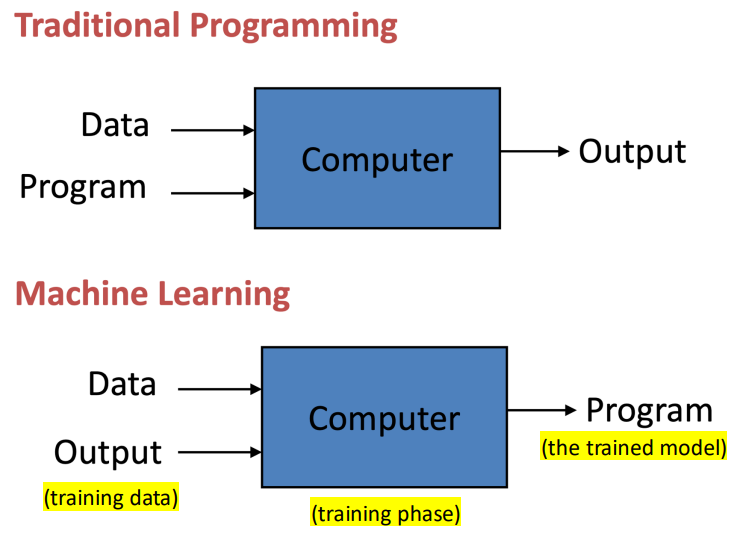
\includegraphics[width=0.4\linewidth]{images/eeai6.png}
    \caption{Traditional programming and Machine Learning}
\end{figure}
\noindent An essential aspect of Machine Learning is choosing the right model for the task. 
We aim to select a model that minimizes the error when classifying the training data. 
Models can belong to various families, such as linear or polynomial models, neural networks, and more.

\subsection{Supervised Learning}
Let's consider a simple two-dimensional problem. 
Designing a classifier requires us to identify a function that separates the labeled data points. 
Some key aspects to focus on include:
\begin{itemize}
    \item Linear or nonlinear approaches. 
    \item The number of points available or the total number of points. 
    \item The choice of technique for designing the classifier.
\end{itemize}

\paragraph*{Regression}
In nonlinear regression, given a set of noisy data points $(x_i,y_i)$, the goal is to reconstruct the underlying function. 
This is expressed as:
\[y(x,\mathbf{w})=\sum_{j=0}^{M}w_jx^j\]
\noindent To train the model, we minimize the Residual Sum of Squares with the following formula:
\[\mathcal{L}(\mathbf{w})=\dfrac{1}{2}\sum_{n=1}^N\left(y(x_n,\mathbf{w})-t_n\right)^2\]
Here, $y(x_n,\mathbf{w})$  is the model's output for the input sample $x_n$, $x_n$ represents the input data, and $t_n$ is the target value (the expected output for a given input).

\subsection{Training}
The training error isn't always reliable because it only measures the performance of the model on the data used for training. 
To get a better understanding of how well the model generalizes, we need to split the dataset into a training set and a test set, ensuring that the model isn't tested on the same data it was trained on.

Typically, the test error will be higher than the training error, as the model is being evaluated on unseen data. 
The amount of data we have plays a crucial role in determining the final quality of the model (more data generally leads to better results).

Additionally, we can introduce a validation set. 
This allows us to adjust the complexity of the model based on the available data, helping to avoid overfitting or underfitting the model to the training data.

\paragraph*{Model complexity}
The complexity of a model, denoted by $M$, plays a crucial role in its performance.
If the model is too complex for the available data, it will overfit (it learns the training data too well, including noise, which leads to poor generalization and weak performance on new data).
On the other hand, if the model is too simple, it won't capture all the important patterns in the data, leading to high error even on the training set. This is known as underfitting.
To achieve the best performance on both training and testing data, we must find an optimal model complexity that balances these two extremes.

\paragraph*{Number of samples}
Additionally, the number of samples, $N$ significantly impacts the model's reliability. 
If we have too few samples, the model may fail to generalize properly, making it difficult to learn the correct patterns.

\paragraph*{Error}
The total error in a learning model is composed of three main components:
\[\text{error} = \text{approximation error} + \text{estimation error} + \text{inherent error}\]
\noindent Here, we have: 
\begin{itemize}
    \item \textit{Approximation error}: this occurs when the learning algorithm does not find the best possible model within the chosen hypothesis space. 
        In other words, it's the difference between the best theoretical model within our chosen framework and the actual model we obtain due to limitations in data or training.
    \item \textit{Estimation error}: this arises when the chosen model family (or hypothesis space) does not perfectly match the true data-generating process. 
        It represents the error introduced by selecting a model class that may not include the optimal solution.
    \item \textit{Inherent error}: this error is unavoidable as it stems from the complexity and noise in the data itself. 
        It depends on the fundamental nature of the learning problem and can only be reduced by improving data quality or redefining the problem. 
\end{itemize}
\noindent Reducing both approximation and estimation errors is key to improving model performance, while inherent error is often a fundamental limitation of the problem itself.

\subsection{Validation}
To properly evaluate a machine learning model, we divide the dataset into three parts: 
\begin{itemize}
    \item \textit{Training set}: used to train the model by adjusting its parameters.
    \item \textit{Validation set}: used to tune hyperparameters and prevent overfitting.
    \item \textit{Test set}: used to assess the final model's performance on unseen data.
\end{itemize}
\noindent When evaluating a classifier, we use the confusion matrix, which summarizes the model's performance by comparing predicted and actual class labels:
\renewcommand{\arraystretch}{1.5}
\begin{table}[h]
    \centering
    \begin{tabular}{|c|cc|}
        \hline
         & \textbf{Predicted positive} & \textbf{Predicted negative} \\
        \hline
        \textbf{Actual positive} & TP (True Positive) & FN (False Negative) \\
        \textbf{Actual negative} & FP (False Positive) & TN (True Negative) \\ 
        \hline
    \end{tabular}
    \caption{Confusion matrix}
\end{table}
\renewcommand{\arraystretch}{1}

\noindent Here, the total number of samples is:
\[N=\text{TP}+\text{TN}+\text{FP}+\text{FN}\]
\noindent From this matrix, we can derive key performance metrics:

\begin{itemize}
    \item \textit{Accuracy}: measures overall correctness but can be misleading for imbalanced datasets: 
        \[\text{accuracy}=\dfrac{\text{TP}+\text{TN}}{N}\]
    \item \textit{Receiver Operating Characteristics}: plots the True Positive Rate against the False Positive Rate. 
        The classifier's performance is represented as a point on this curve. 
        Changing the classification threshold alters this position. 
        A diagonal line corresponds to random guessing, and any performance below this line implies systematically incorrect predictions.  
\end{itemize}

\paragraph*{Model validation}
To validate a model we can use various techniques: 
\begin{itemize}
    \item \textit{Apparent Error Rate}: the entire dataset $Z_N$ is used for both training and error estimation. However, this method often underestimates the true error due to overfitting.  
    \item \textit{Sample Partitioning}: the dataset $Z_N$ is randomly split into two disjoint subsets: $S_D$, used for training, and $S_E$, used for evaluation.  
    \item \textit{Leaving-One-Out}: improves upon this by iterating over the dataset $N$ times. 
        Each time, one sample is left out for evaluation while the remaining $N-1$ samples are used for training. 
        The final estimate is obtained by averaging all $N$ iterations.  
    \item \textit{$k$-fold Cross Validation}: the dataset is randomly divided into $k$ disjoint subsets of equal size. 
        For each subset, the remaining $k-1$ subsets form the training set $S_D$, while the reserved subset is used as the evaluation set $S_E$. 
        The process repeats $k$ times, and the results are averaged. This approach generalizes LOO and reduces variance when $k \ll N$.  
\end{itemize}
\noindent By carefully selecting the validation method, we can ensure a more reliable assessment of the model’s performance while minimizing bias and variance.

\subsection{Neural Networks}
Neural networks are mathematical models designed to capture relationships in space, time, and the state of individual neurons. 
Each neuron processes input data through a weighted sum:
\[a_t=\sum_{i=1}^{m}x^iw^i\]
\noindent This scalar product measures the affinity between input values and weights. 
Before activation, it represents the neuron's raw output. An activation function is then applied to introduce non-linearity and determine the final neuron output.

A typical neural network consists of an input layer, one or more hidden layers, and an output layer.
Training a neural network involves minimizing a loss function. 
For a Feed Forward Neural Network, a common loss function is the Residual Sum of Squares:
\[\mathcal{L}(\mathbf{w})=\dfrac{1}{2}\sum_{n=1}^{N}\left(y(\mathbf{x}_n,\mathbf{w})-t_n\right)^2\]
Since this function lacks a closed-form solution due to its non-linearity, optimization techniques such as Stochastic Gradient Descent (SGD) are used to iteratively update weights:
\[\mathbf{W}^{(t+1)}=\mathbf{w}^{(t)}-\eta\nabla\mathcal{L}(\mathbf{w}^{(t)})\]
\noindent Here, $\eta$ represents the learning rate, controlling the step size in the direction of the gradient $\nabla\mathcal{L}(\mathbf{w}^{(t)})$. 
The goal is to find the best possible local minimum, as computing the global minimum is often infeasible.

\begin{theorem}
    A Feed Forward Neural Network with a single hidden layer containing a finite number of neurons can approximate any continuous function defined on compact subsets.
\end{theorem}
\noindent This theorem implies that, in theory, a properly configured neural network can achieve zero approximation error for any target function. 
However, in practice, finding the exact network that achieves this perfect approximation is extremely challenging.

\paragraph*{Memory demand}
The memory required by a Feed Forward Neural Network depends on the number of layers and the number of connections within each layer. 
Every connection between neurons has an associated weight, and each neuron also has a bias, which is another weight that needs to be stored.
For a given layer, the total memory demand for weights can be calculated using the following formula:
\[\text{weights}=\sum_{l=1}^{L}=(N_l\cdot N_{l-1}+N_l)\]
Here, $L$ is the total number of layers (excluding the input layer), $N_l$ is the number of neurons in layer $l$, $N_{l-1}$ is the number of neurons in the previous layer. 
This formula gives the total number of weights that must be stored in memory. 
If each weight is stored using a specific precision, the total memory demand can be computed by multiplying the number of weights by the storage size per weight.